\documentclass[a4paper,11pt]{article}

% Indent below title
\usepackage{indentfirst}
% Line spacing
\usepackage{setspace}
% Todo notes
\usepackage{todonotes}
% Mathematics symbols
\usepackage{amsmath}
\usepackage{amssymb}
\DeclareMathOperator*{\argmin}{argmin}
% Figures
\usepackage{graphicx}
\usepackage{subfig}
\usepackage{placeins}
\graphicspath{ {./images/} }
% Links
\usepackage[
colorlinks=true,
linkcolor=blue,
urlcolor=blue,
citecolor=black
]{hyperref}
% Tables
\usepackage{tabularx}
\usepackage[thinlines]{easytable}
% Units
\usepackage{siunitx}
% References
\usepackage[style=apa, backend=biber]{biblatex}
\addbibresource{sections/references.bib}
% Hyphen
\usepackage{hyphenat}

\begin{document}

\thispagestyle{empty}

\begin{spacing}{1}
    \centering
    \large Vanier College\\
    \large Faculty of Science and Technology\\
    \large Department of Physics\\
    \vspace{1cm}
    \Large\textbf{Implementing SLAM and Autonomous Navigation on a TurtleBot3}\\
    \vspace{1cm}
    \large Vu Dang Khoa Chiem (6196555)\\
    \vspace{1cm}
    \large Presented to Prof. Jicai Pan\\
    \large Statics and Engineering Physics (203-HTK-05 sect. 00002)\\
    \large May 12, 2024
\end{spacing}

\begin{abstract}
    This paper serves as an introduction to understanding Simultaneous Localization and Mapping (SLAM) and autonomous navigation in the ROS2 framework using a TurtleBot3 robot. It provides an analysis of the underlying mathematical foundations and algorithms used. As autonomous robots become ubiquitous in society, the need for robust and efficient SLAM techniques is critical. Achieving autonomous navigation involves several key steps. First, a map of the environment needs to be pre-generated \parencite{hessRealtimeLoopClosure2016}. The robot's 360° LiDAR sensor generates scans that are processed and optimized to create submaps. These submaps are then stitched together into a complete map of the environment using a loop-closing optimization. Second, localization is done using Adaptive Monte Carlo Localization (AMCL), which employs a particle filter to estimate the robot's pose (position and orientation) in the environment probabilistically \parencite{thrunProbabilisticRobotics2006}. Third, the map previously built is transformed into a layered cost map \parencite{macenskiDesksROSMaintainers2023}. This cost map inflates obstacles and dynamically considers new ones. By expanding a wavefront from the goal to the robot's starting position, this cost map is transformed into a navigation function represented by wavefront crossing times on the grid map \parencite{philippsenInterpolatedDynamicNavigation2005}. The global path planner (Navigation Function planner), using a gradient descent approach, optimizes the navigation function to find the fastest path to the desired goal location. Fourth, by estimating linear and angular velocities, the local path planner uses the Dynamic Window Approach (DWA) to repeatedly generate small circular arcs that follow the global path \parencite{macenskiDesksROSMaintainers2023}. Altogether, while there are still bugs to be fixed, the robot is able to navigate autonomously.
\end{abstract}

\filbreak

\renewcommand{\abstractname}{Résumé}
\begin{abstract}
    En analysant les principes mathématiques et les algorithmes utilisés, cet article sert d'introduction à la localisation et cartographie simultanées (SLAM) et à la navigation autonome dans ROS2 à l'aide d'un robot TurtleBot3. Comme les robots autonomes deviennent progressivement plus communs dans la société, le besoin de techniques SLAM robustes et efficaces est essentiel. La navigation autonome implique plusieurs étapes clés. Premièrement, une carte de l'environnement doit être pré-générée \parencite{hessRealtimeLoopClosure2016}. Le capteur LiDAR 360° du robot génère des scans qui sont transformés en sous-cartes. Celles-ci sont ensuite assemblées pour former une carte complète de l'environnement avec une optimisation de fermeture de boucle. Deuxièmement l'algo\hyp{}rithme Adaptive Monte Carlo Localization (AMCL), qui estime des distributions de probabilité avec des particules, est utilisé pour estimer la position et l'orientation du robot dans l'environnement \parencite{thrunProbabilisticRobotics2006}. Troisièmement, la carte précédemment construite est transformée en une carte de coûts qui gonfle les obstacles et considère les nouveaux qui apparaissent \parencite{macenskiDesksROSMaintainers2023}. En propageant une onde de l'objectif jusqu'à la position de départ du robot, cette carte de coûts est transformée en une fonction de navigation représentée par des temps de passage de l'onde sur la grille \parencite{philippsenInterpolatedDynamicNavigation2005}. Le planificateur global de chemin (Navigation Function Planner), utilisant une approche de descente de gradient, optimise la fonction de navigation pour trouver le chemin le plus rapide vers l'emplacement souhaité. Quatrièmement, en estimant les vitesses linéaires et angulaires, le planificateur local de chemin utilise l'approche par fenêtre dynamique (DWA) pour générer de manière répétée de petits arcs de cercle qui suivent le chemin global \parencite{macenskiDesksROSMaintainers2023}. Bref, même s'il reste encore des bogues à régler, le robot peux naviguer de manière autonome.
\end{abstract}


\newpage

\section{Introduction} \label{introduction}
This project aims to implement a Simultaneous Localization and Mapping (SLAM) algorithm on a TurtleBot3 Waffle Pi robot using the Robot Operating System 2 (ROS2) framework for the purpose of autonomous environment mapping, localization, and navigation. In other words, the goal will be for the robot to move in an environment from one point to another while avoiding obstacles. SLAM is important for autonomous vehicles as it allows a vehicle to map a room and localize itself in it at the same time.

This paper utilizes a variety of robotics terminology. The term ``pose'' refers to an object's position and orientation in space, typically represented by a three-dimensional vector ($x,y,\theta$) \parencite{corkeRoboticsVisionControl2023}. Odometry encompasses the measurements of an object's travel distance and direction, often achieved through the use of wheel encoders. Dead reckoning is the process of estimating an object's pose based on the information obtained from odometry data. Put differently, this navigation method doesn't rely on any observations of the environment.

Many optimization algorithms are used in this project. These algorithms often need to use the gradient to iteratively optimize functions. For a multivariable function, the gradient at a given point is a vector with a direction pointing in the direction of fastest increase and a magnitude representing the slope in that direction \parencite{Gradient2024}. For a point $p = (x_1,\hdots, x_n)$ in $\mathbb{R}^n$, the gradient is given by
\[
    \nabla f(p)=\begin{bmatrix}
        \frac{\partial f}{\partial x_1}(p) \\[6pt]
        \vdots                             \\[6pt]
        \frac{\partial f}{\partial x_n}(p)
    \end{bmatrix}.
\]

As of the time of writing this paper, the robot is able to map and localize itself in its environment. There is still an issue with the global path planner due to over-inflation of the obstacles, but it can be fixed by changing the inflation parameters. Otherwise, when dead reckoning to a target position, a significant discrepancy between the estimated and actual robot location is observed. This is caused by wheel slippage and velocities being rounded to 0.

\section{Setup} \label{setup}
As shown in Figure \ref{fig:turtlebot3}, the TurtleBot3 is equipped with many components, including a Raspberry Pi 4 (small computer) for onboard processing, a differential drive system, and a 360° 2D LiDAR sensor for observations. Due to the limitations of the onboard computer, the robot (client) relies on an external computer (server) for most processing tasks. The server processes data obtained by the robot's LiDAR sensor and transmits control parameters back to it at very fast regular intervals. These control parameters are the linear and angular velocities ($v,\omega$) of the robot that control the differential drive system. This driving system consists of two wheels, one on each side, that can be controlled independently, allowing the robot to turn by having one wheel turn more slowly than the other \parencite{corkeRoboticsVisionControl2023}. The LiDAR sensor, which constantly rotates to observe around the robot, measures distances by ``[emitting] short pulses of infrared laser light and [measuring] the time for the reflected pulses to return'' \parencite{corkeRoboticsVisionControl2023}.

\begin{figure}[!htb]
    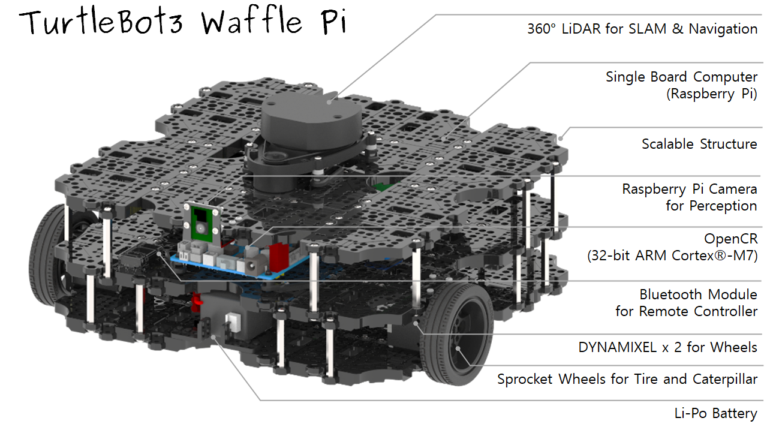
\includegraphics[width=8cm]{turtlebot3.png}
    \centering
    \caption{Components of the TurtleBot3 Waffle Pi \parencite{ROBOTISEManual}.}
    \label{fig:turtlebot3}
\end{figure}

A few essential pieces of software are used for the development of the robot. Firstly, as ROS2 Humble best supports the Ubuntu 22.04 LTS (Jammy Jellyfish) Linux distribution, this operating system is used to code and control the robot \parencite{InstallationROSDocumentation}. The use of ROS2 allows the robot to be programmed using a combination of both Python and C++. Secondly, Gazebo Ignition Fortress is used to simulate and visualize the robot in a 3D environment. This allows writing and testing on a virtual robot without the need for real robot hardware, which facilitates collaboration between students and remote development. Thirdly, RViz is used to control the robot and visualize the cost map.

\section{Mapping} \label{mapping}
To effectively localize and navigate itself, the robot's algorithm first needs a map of its environment. This map consists of a probability grid with each square enclosing an area of \qty{5}{cm^2} in the real-world \parencite{hessRealtimeLoopClosure2016}. Since the map is formatted as a grayscale image file (PGM), the squares are referred to as pixels. Each pixel is assigned a value between 0 (white) and 1 (black), representing the probability of the pixel being occupied. A probability closer to 0 means the square is likely to be empty, while a probability closer to 1 means the square is likely to be occupied. An example map is shown in Figure \ref{fig:map}.

\begin{figure}[!htb]
    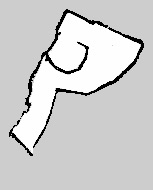
\includegraphics[width=4cm]{map.jpeg}
    \centering
    \caption{A grayscale map generated by a TurtleBot3.}
    \label{fig:map}
\end{figure}

\subsection{Building Submaps} \label{submaps}
The complete map of the environment is built by stitching multiple submaps together \parencite{hessRealtimeLoopClosure2016}. Each submap is built using a few consecutive LiDAR scans by aligning their coordinate frames. This project uses six scans per submap, but this parameter can be changed. The matrix transformation used to rotate counterclockwise and translate the scan on the XY-plane is given by
\[
    T_\xi p =
    \begin{bmatrix}
        \cos(\xi_\theta) & -\sin(\xi_\theta) \\
        \sin(\xi_\theta) & \cos(\xi_\theta)
    \end{bmatrix}p + \begin{bmatrix}
        \xi_x \\
        \xi_y
    \end{bmatrix},
\]
where $p$ is a hit point on the scan and $\xi=(\xi_x,\xi_y,\xi_\theta)$ is the scan's pose relative to the submap \parencite{RotationMatrix2024,hessRealtimeLoopClosure2016}. All the hit points in a single scan can be represented as $H=\{h_k\}_{k=1,\ldots,K},h_k\in\mathbb{R}^2$. In order to determine the pose of each scan, a scan matcher is used to ``[maximize] the probabilities at the scan points in the submap'' \parencite{hessRealtimeLoopClosure2016}. This ensures the best possible alignment and overlap between the scans in a submap. An optimizer, such as the Ceres Solver, is used to optimize the non-linear least squares problem
\[
    \argmin_{\xi} \sum_{k=1}^{K}(1 - M_\text{smooth}(T_\xi h_k))^2
\]
\parencite{SolvingNonlinearLeast,hessRealtimeLoopClosure2016}. Here, ``$T_\xi$ transforms [each hit point on a scan ($h_k$)] from the scan coordinate frame to the submap coordinate frame'' \parencite{hessRealtimeLoopClosure2016}. The $M_\text{smooth}$ function interpolates the discrete probabilities of each pixel in the submap into a continuous curve with bicubic interpolation, as shown in Figure \ref{fig:bicubic}. By plugging the transformed point into $M_\text{smooth}$, the current occupancy probability in the submap at that point is obtained. Thus, $1 - M_\text{smooth}(T_\xi h_k)$ represents the difference between the scan's probability and the submap's probability at that point. The square serves to amplify large differences and reduce small differences. By minimizing the sum of all these differences, the $\argmin$ function identifies the pose ($\xi$) that aligns the scan data most optimally with the existing submap, maximizing their overlap. Initially, this pose ($\xi$) can be estimated using the robot's odometry through dead reckoning.

\begin{figure}[!htb]
    \centering
    \subfloat[\centering Non-interpolated]{{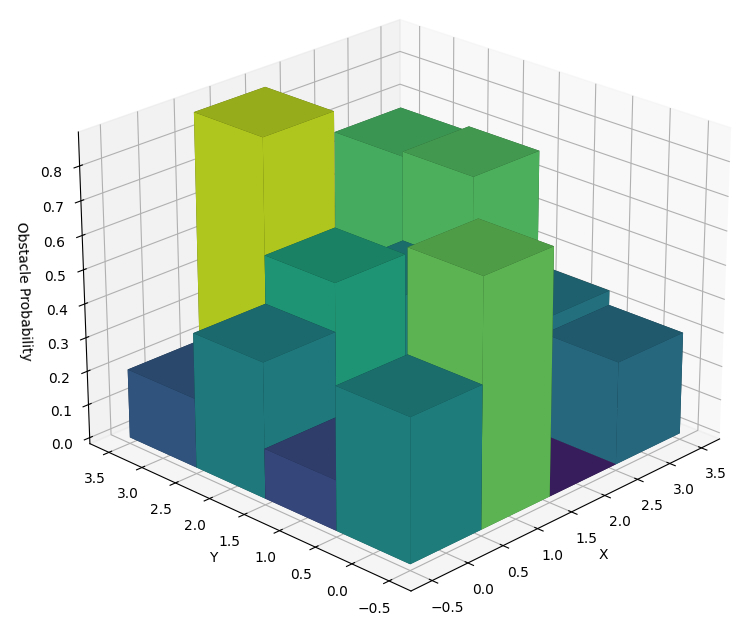
\includegraphics[width=5cm]{bicubic-ni} }}
    \qquad
    \subfloat[\centering Bicubic interpolation]{{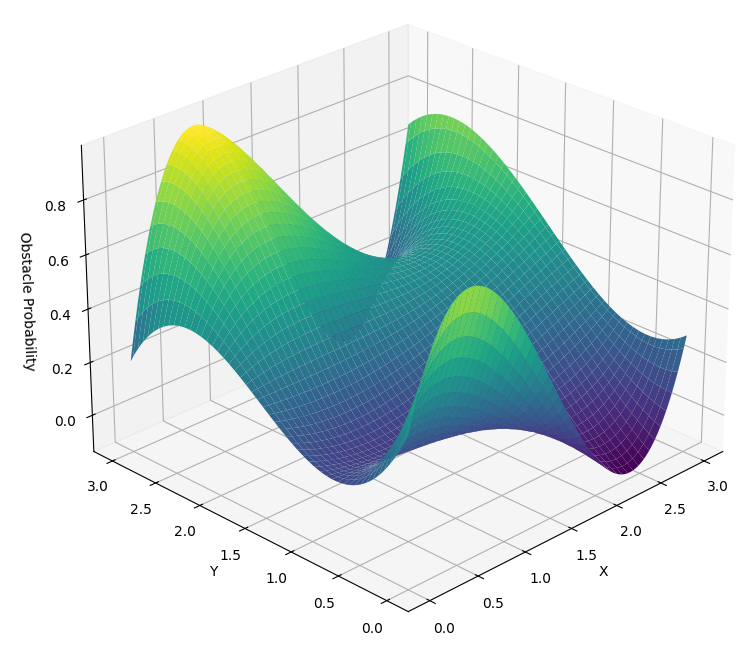
\includegraphics[width=5cm]{bicubic-bi} }}
    \caption{3D representation of the bicubic interpolation done by $M_\text{smooth}$ for a small submap.}
    \label{fig:bicubic}
\end{figure}

To insert a scan into a submap, each pixel that intersects a hit point is added to a ``hits'' list, and each pixel situated on the straight path from the robot's LiDAR sensor to a hit point, except for the ones also intersecting another hit point, is added to a ``misses'' list \parencite{hessRealtimeLoopClosure2016}. A probability value between 0 and 1 is then assigned to each pixel in both lists. If a pixel was never observed before in the submap, it is assigned a predefined probability of $p_{hit}$ or $p_{miss}$ depending on which list it is in. If a pixel was already observed, its old probability ($M_\text{old}$) can be updated by calculating a new probability ($M_\text{new}$) using the function
\[
    M_\text{new}(x)=clamp(odds^{-1}(odds(M_\text{old}(x))\cdot odds(p_\text{hit/miss}))),
\]
where $odds(p)=\frac{p}{1-p}$ and $odds^{-1}(p)=\frac{p}{1+p}$. The clamp function restricts probabilities to a predefined range to avoid issues with the $odds$ function and prevent the robot from treating cells with absolute certainty due to sensor errors. Given a scenario where $p_{hit}=0.750$ and a hit point intersects with an already observed pixel currently having a probability of 0.700, the new probability can be calculated as follows:
\begin{enumerate}
    \item $odds(p)=odds(0.75)=\frac{0.750}{1-0.750}=3.00$
    \item $odds(p)=odds(0.7)=\frac{0.700}{1-0.700}=2.33$
    \item $M_\text{new}(x)=clamp(odds^{-1}((2.33)(3.00)))=clamp(odds^{-1}(7.00))=\frac{7.00}{1+7.00}=0.875$
\end{enumerate}
Now, the probability of this pixel is changed to 0.875.

\subsection{Building a Map} \label{map}
By focusing solely on a few recent scans for submap creation, this method can slowly drift away from an accurate representation of the environment due to accumulated errors \parencite{hessRealtimeLoopClosure2016}. Hence, a second scan matcher runs to compare scans between submaps that overlap. When a match is identified, ``the... [estimated] relative pose [of the scan in its submap] is added to the optimization problem'' \parencite{hessRealtimeLoopClosure2016}. In other words, a constraint is added to stitch the submaps together. This loop closure optimization runs every few seconds to repair the accumulated error when the robot revisits a position. An optimizer, such as the Ceres Solver, can be used to solve the following non-linear least squares problem
\[
    \argmin_{\Xi^\text{m},\Xi^\text{s}} \frac{1}{2}\sum_{ij}\rho(E^2(\xi_i^\text{m},\xi_j^\text{s};\Sigma_{ij},\xi_{ij})),
\]
where $\Xi^\text{m}=\{\xi_i^\text{m}\}_{i=1,\ldots,m}$ are the submap poses, $\Xi^\text{s}=\{\xi_j^\text{s}\}_{j=1,\ldots,n}$ are the scan poses, and $\xi_{ij}$ is a relative pose constraint added by the second scan matcher \parencite{SolvingNonlinearLeast,hessRealtimeLoopClosure2016}. $\Sigma_{ij}$, which is estimated by the optimizer, is a covariance matrix associated with $\xi_{ij}$. A covariance matrix is a square matrix that describes the variance of individual variables (dispersion of data) and the covariance between pairs of variables (how the variables vary together) \parencite{CovarianceMatrixFormula}. In this case, it is used to estimate the uncertainty of $\xi_{ij}$. $\rho$ is a loss function used to minimize the impact of incorrect constraints added during the scan matching. The $E^2$ function is given by
\[
    E^2(\xi_i^\text{m},\xi_j^\text{s};\Sigma_{ij},\xi_{ij})=e(\xi_i^\text{m},\xi_j^\text{s},\xi_{ij})^T\Sigma_{ij}^{-1}e(\xi_i^\text{m},\xi_j^\text{s},\xi_{ij}),
\]
where $e(\xi_i^\text{m},\xi_j^\text{s},\xi_{ij})=\xi_{ij}-\begin{bmatrix}
        R_{\xi_i^\text{m}}^{-1}(t_{\xi_i^\text{m}}-t_{\xi_j^\text{s}}) \\
        \xi_{i;\theta}^\text{m}-\xi_{j;\theta}^\text{s}
    \end{bmatrix}$. The $E^2$ function computes the squared error between the estimated and actual scan pose in its submap. Thus, the loop closure optimization attempts to minimize this error.

\section{Localization} \label{localization}
Adaptive Monte Carlo Localization (AMCL) is used by the robot to localize itself in the environment \parencite{thrunProbabilisticRobotics2006}. This algorithm considers three types of robot data which change at repeating short time intervals: states, control parameters, and measurements. A state is the pose of the robot at a time interval ($x,y,\theta$) and the fixed environment grid map. Control parameters are the linear and angular velocities ($v,\omega$) executed by the robot between two time intervals. A measurement is the hit points gathered by the robot's LiDAR sensor during a time interval.

The robot's current state is assumed to be a result of all its past states, movements, and observations. Therefore, the robot's past and future are independent of each other, as described by the Markov property \parencite{MarkovProperty2024a}. The probability of a future state depends solely on the current state since it encompasses all the required information. Thus, the current state and the next movement can be used to predict the new state of the robot after the movement \parencite{thrunProbabilisticRobotics2006}. Then, using this new state, the next noisy measurements can also be predicted. This generative model is called the hidden Markov model (HMM) \parencite{thrunProbabilisticRobotics2006}.

The robot's pose in the global map coordinate system cannot be measured directly \parencite{matlabUnderstandingParticleFilter2020,thrunProbabilisticRobotics2006}. Hence, the current pose needs to be found using past movements and measurements. Due to uncertainties in the measurements, the AMCL algorithm estimates the pose using a probabilistic approach instead of a deterministic one. Thus, probability distributions, called beliefs, need to be used to predict the pose. In the context of this project, a particle filter is used by ROS2 to represent the beliefs. This works by placing more than 1000 particles, representing possible robot states, randomly on areas of belief and updating it at each time interval. In the beginning, the probability of the robot's pose is the same everywhere, so particles are generated randomly everywhere on the map; however, as the robot moves in the environment, more data is gathered, and the particles become increasingly concentrated in new areas of belief, as shown in Figure \ref{fig:belief}. Therefore, as the belief becomes more precise, progressively fewer particles are needed, increasing the efficiency of the program.

\begin{figure}[!htb]
    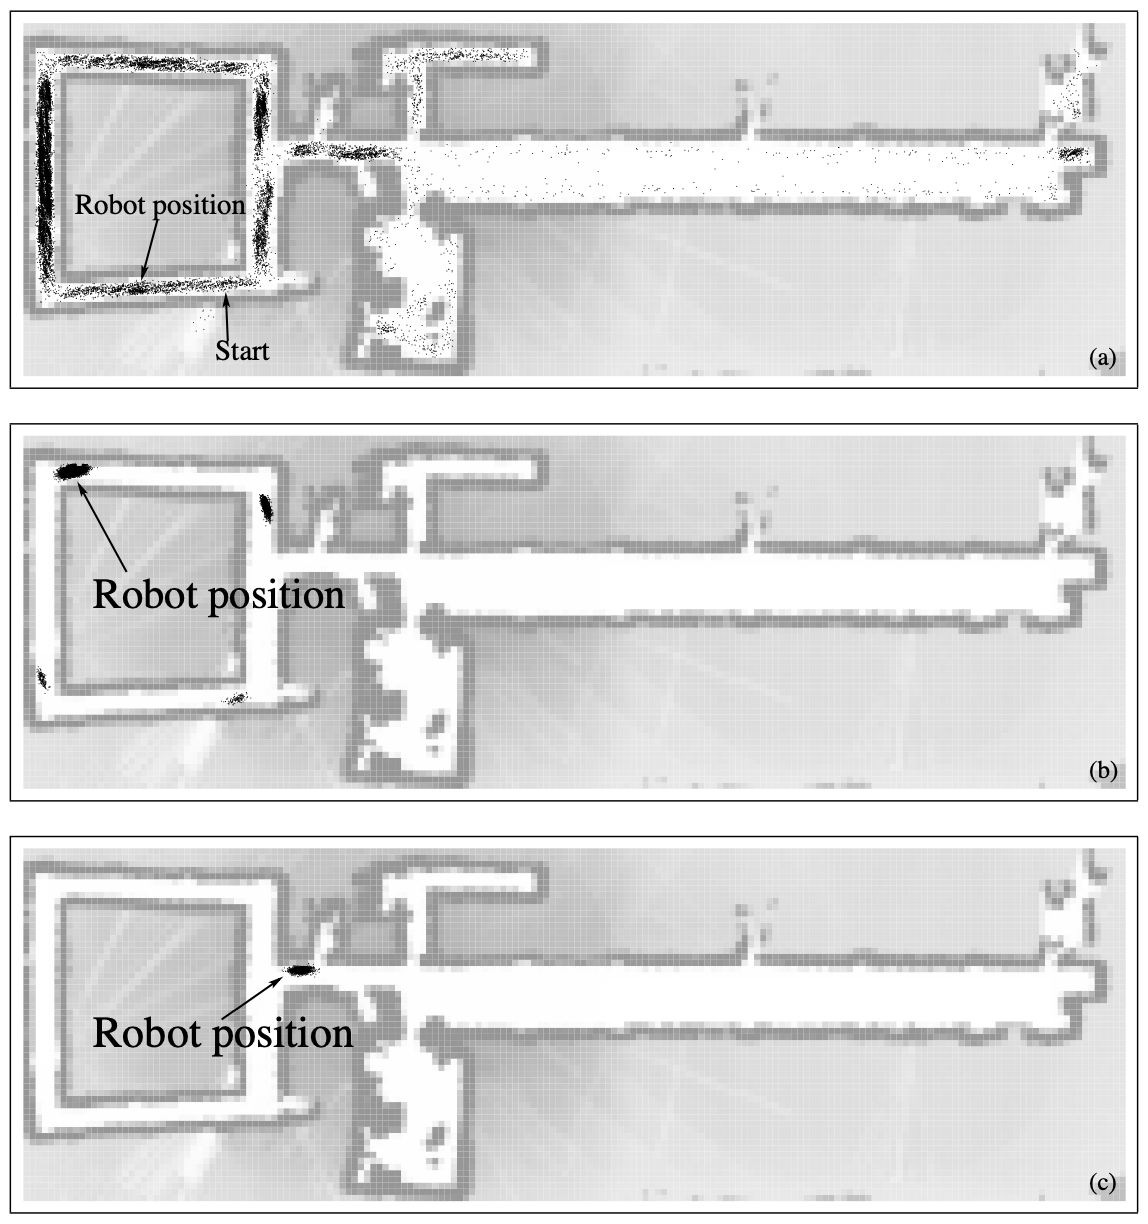
\includegraphics[width=8cm]{AMCL}
    \centering
    \caption{Change in the probability distribution of a robot's position (belief) with time \parencite{thrunProbabilisticRobotics2006}. In Adaptive Monte Carlo Localization (AMCL), this distribution is approximated by a set of particles, each representing a possible robot pose. While each particle also has an associated direction, it's omitted from the figure due to clutter.}
    \label{fig:belief}
\end{figure}
\filbreak
%\todo{May need some work}

\section{Navigation} \label{navigation}
\subsection{Building a Cost Map} \label{cost-map}
The robot uses a cost map to navigate its environment. Similar to the map described in section 2.2, it is a grid of squares, each representing a \qty{5}{cm^2} area in the real-world \parencite{macenskiDesksROSMaintainers2023}. Each square is assigned a cost: an integer ranging from 0 to 255. The higher the cost, the harder it is for the robot to cross that square; thus, the pathfinding algorithm finds a path with the lowest cost. There are two special integers: 254 signifies impassable squares, and 255 indicates unknown squares.

This cost map, called Layered Costmap, is generated by stacking multiple dynamic layers originating from different sources \parencite{macenskiDesksROSMaintainers2023}. Periodically, the cost map is updated by refreshing the layers with new sensor measurements. ROS2 provides many layers by default:
\begin{enumerate}
    \item \textbf{Static layer}: This layer is a pre-built map of the environment, typically created by manually navigating the robot and collecting sensor data (as described in section \ref{map}). It is accessed by ``[subscribing] to an OccupancyGrid topic'' \parencite{macenskiDesksROSMaintainers2023}. Due to continuous mapping, this map can evolve over time, capturing changes in the environment.
    \item \textbf{Obstacle layer}: Using the highly accurate LIDAR sensor, this layer detects the immediate obstacles around the robot. The hit points measured by the sensor are treated with absolute certainty. The robot assumes there is empty space between itself and any hit point it measures.
    \item \textbf{Inflation layer}: Based on occupancy data of other layers, this layer adds a safety buffer zone around obstacles to prevent collisions. For a given square located at ($x,y$) in the map close to an obstacle, its cost is increased using the equation
          \[
              cost(x,y)=(cost_\text{lethal}-1)e^{-\omega_{scale}(d_0-r)},
          \]
          where ``$d_0$ is the distance [from square ($x,y$)] to the [nearest] obstacle, $cost_\text{lethal}$ is the [cost of that nearest obstacle], and $r$ is the [robot's] inscribed radius...'' \parencite{macenskiDesksROSMaintainers2023}. The cost scaling factor ($\omega_{scale}$) is a constant that controls the steepness of cost increase around obstacles. A higher value will result in a steeper increase.
    \item \textbf{Keepout layer}: This layer can increase the cost of certain squares using input masks, even if there are no obstacles. It is used to make the robot avoid certain areas.
    \item \textbf{Speed layer}: This layer can define zones with specific speed restrictions. It is used to make the robot slow down in certain areas.
\end{enumerate}
An example cost map is shown in Figure \ref{fig:rviz}.

\begin{figure}[!htb]
    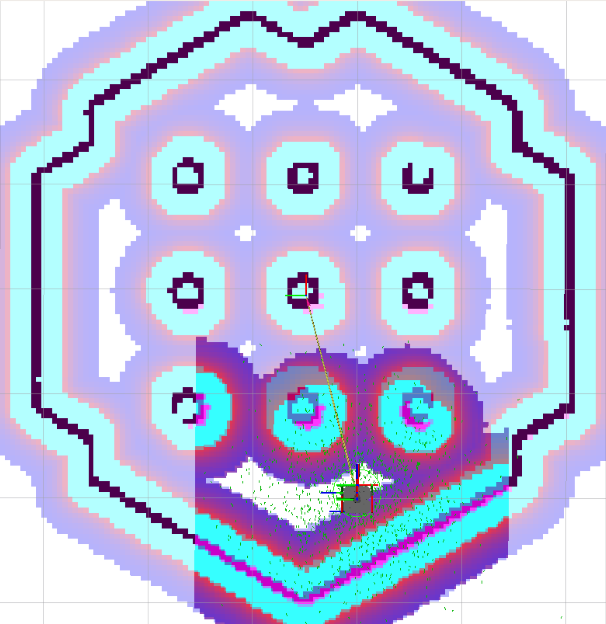
\includegraphics[width=8cm]{rviz.png}
    \centering
    \caption{Example cost map displayed by RViz.}
    \label{fig:rviz}
\end{figure}
\FloatBarrier

\subsection{Dijkstra's Algorithm} \label{dijkstra}
Dijkstra's algorithm is used to find the shortest path between two points in a network of nodes \parencite{computerphileDijkstraAlgorithmComputerphile2017}. As an example, consider the network shown in Figure \ref{fig:dijkstra}a. The goal is to find the shortest path from node A to node E. The following steps outline how to solve this problem using Dijkstra's algorithm.

\begin{figure}[!htb]
    \centering
    \subfloat[\centering Shortest path is unknown] {{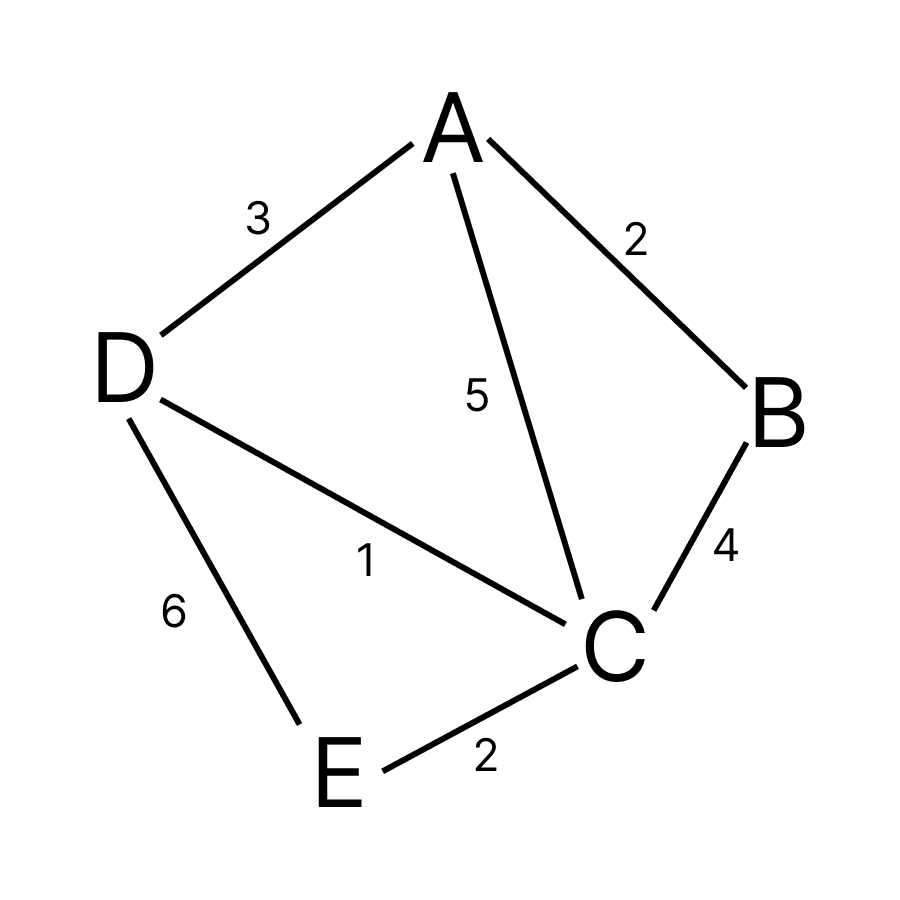
\includegraphics[width=5cm]{dijkstra1} }}
    \qquad
    \subfloat[\centering Shortest path is found]{{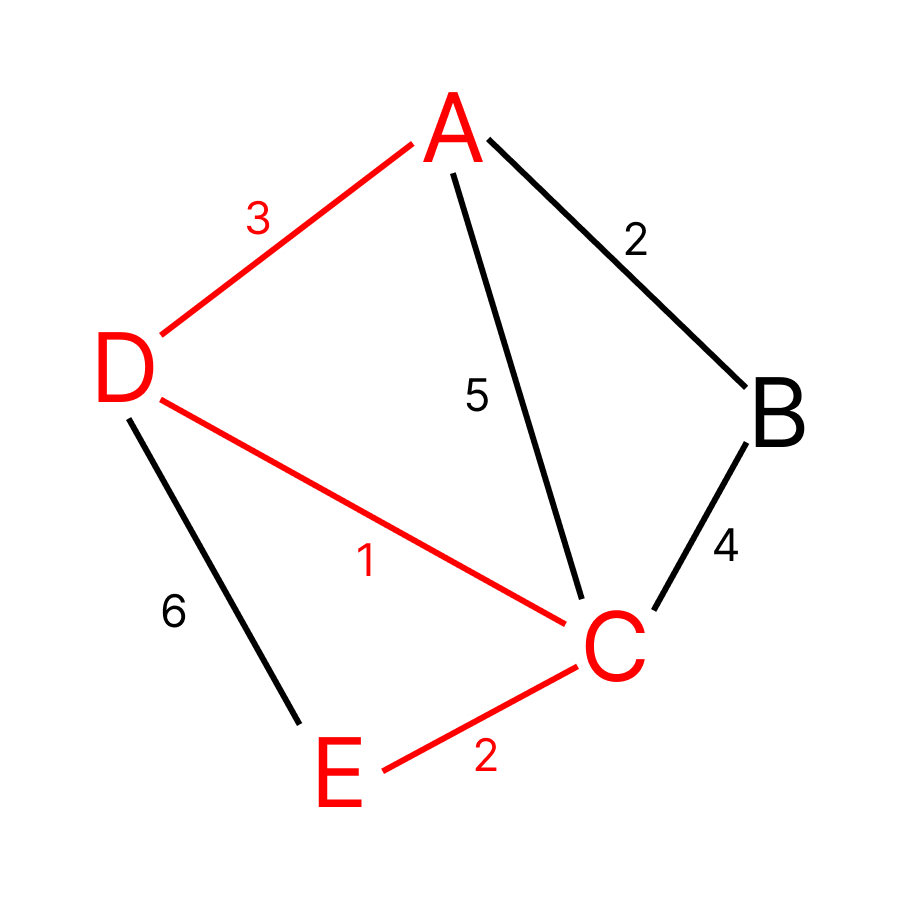
\includegraphics[width=5cm]{dijkstra2} }}
    \caption{Example of a network of nodes where the goal is to find the shortest path from node A to node E.}
    \label{fig:dijkstra}
\end{figure}

\filbreak

\begin{enumerate}
    \item \textbf{Current node: A}\\
          $\text{closed} = \{A\}$\\
          \def\arraystretch{1.5}
          \begin{tabular}{ |c|c|c|c|c|c|c|c| }
              \hline
                             & A & B & C & D & E        \\
              \hline
              Distance ($d$) & 0 & 2 & 5 & 3 & $\infty$ \\
              \hline
              Previous node  & - & A & A & A & A        \\
              \hline
          \end{tabular}
    \item \textbf{Current node: B}\\
          Since B is the closest node to A, it is added to the closed list.\\
          $\text{closed} = \{A,B\}$
          \begin{itemize}
              \item $d_C=\min(5,2+BC)=\min(5,2+4)=\min(5,6)=5$
              \item $d_D=\min(3,2+BD)=\min(3,2+\infty)=\min(3,\infty)=3$
              \item $d_E=\min(\infty,2+BE)=\min(\infty,2+\infty)=\min(\infty,\infty)=\infty$
          \end{itemize}
          Since there are no changes in the distance values, travelling from A to B directly is the shortest distance. Therefore, the previous nodes remain the same.
    \item \textbf{Current node: D}\\
          Node D is added to the closed list because it is the next shortest path.\\
          $\text{closed} = \{A,B,D\}$
          \begin{itemize}
              \item $d_C=\min(5,3+DC)=\min(5,3+1)=\min(5,4)=4$
              \item $d_E=\min(\infty,3+DE)=\min(\infty,3+6)=\min(\infty,9)=9$
          \end{itemize}
          \def\arraystretch{1.5}
          \begin{tabular}{ |c|c|c|c|c|c|c|c| }
              \hline
                             & A & B & C & D & E \\
              \hline
              Distance ($d$) & 0 & 2 & 4 & 3 & 9 \\
              \hline
              Previous node  & - & A & D & A & D \\
              \hline
          \end{tabular}
    \item \textbf{Current node: C}\\
          Node C is added to the closed list because it has the shortest path from D.\\
          $\text{closed} = \{A,B,D,C\}$
          \begin{itemize}
              \item $d_E=\min(9,4+CE)=\min(9,4+2)=\min(9,6)=6$
          \end{itemize}
          \def\arraystretch{1.5}
          \begin{tabular}{ |c|c|c|c|c|c|c|c| }
              \hline
                             & A & B & C & D & E \\
              \hline
              Distance ($d$) & 0 & 2 & 4 & 3 & 6 \\
              \hline
              Previous node  & - & A & D & A & C \\
              \hline
          \end{tabular}
    \item It is possible to find the shortest path by working backwards from E ($E \leftarrow C \leftarrow D \leftarrow A$), as shown in Figure 4b. This path has a length of 6.
\end{enumerate}

\subsection{Global Path Planner} \label{global-planner}
In order for the robot to move towards a goal, a pathfinding algorithm is needed. In this project, the Navigation Function (NavFn) planner plugin from the Nav2 package is used \parencite{NavFnPlannerNav2}. To compute an optimal path to the goal, this plugin uses a potential field called a navigation function. This field acts like a force that guides the robot's movement away from obstacles and towards the goal \parencite{philippsenInterpolatedDynamicNavigation2005}. It is represented by a grid map with each square having a discrete crossing time. As the navigation function is generated, similar to a ripple in water, by propagating a wavefront outwards from the goal until it reaches the robot's starting position, the crossing time is the time at which the wavefront crosses a grid square. The wavefront's position at a time $t$ is given by
\[
    \Gamma (t)=\{(x,y) \mid T(x,y)=t\}.
\]

The potential field is built from the cost map described in section \ref{cost-map}. The costs on the cost map are converted to wavefront propagation speeds ($F$) \parencite{philippsenInterpolatedDynamicNavigation2005}. Due to the cost depicting the difficulty of crossing a grid square, lower costs are converted to higher speeds, while higher costs are converted to lower speeds. The propagation speeds are used to determine the crossing times of the grid squares. If $F(x,y)>0$, the navigation function ($T$) follows the differential equation
\[
    |\nabla T|F=1.
\]
As the navigation function is represented by a discrete grid map, this equation needs to be written in a discrete notation. For a given grid square located at ($i,j$), its crossing time ($T$) can be found using the equation
\begin{equation} \label{eq:discrete-for-navfn}
    \max(D_{ij}^{-x}T,-D_{ij}^{+x},0)^2+\max(D_{ij}^{-y}T,-D_{ij}^{+y},0)^2=\frac{1}{F_{ij}^2},
\end{equation}
where $F_{ij}$ is the propagation speed at the grid square, and each $D_{ij}$ is the difference quotient along its respective axis. The difference quotient, also called Newton's quotient, gives the average rate of change of a function between two points \parencite{DifferenceQuotient2023}. It is given by
\[
    f'(x)\approx\frac{f(x+h)-f(x)}{h}
\]
The true derivative of the function is obtained by taking $\lim\limits_{h\to0}$ of this equation. Looking at equation \ref{eq:discrete-for-navfn}, only two neighbouring squares (located on different axes) at most will be involved in the crossing time computation \parencite{philippsenInterpolatedDynamicNavigation2005}. For example, in the scenario shown in Figure \ref{fig:wavefront-expansion}, supposing that the neighbouring cells are B and C and that $T_B\leqslant T_C$, the quadratic equation to find the crossing time ($T$) of square ($i,j$) is
\begin{equation} \label{eq:crossing-time-quadratic}
    (T-T_B)^2+(T-T_C)^2=\frac{h^2}{F^2},
\end{equation}
where $T_B$ and $T_C$ are the crossing times of the neighbouring squares, h is the size of a square (\qty{5}{cm}), and ``[$F_{ij}$] is the propagation speed at [square] ($i,j$)'' \parencite{philippsenInterpolatedDynamicNavigation2005}. In order to always obtain a real solution for the crossing time ($T$), a fallback quadratic equation is needed; thus, when $T_C-T_A\geqslant h/F$, equation \ref{eq:crossing-time-quadratic} becomes
\[
    (T-T_A)^2=\frac{h^2}{F^2}.
\]
Equation \ref{eq:crossing-time-quadratic} not having a real solution indicates that the wavefront is not able to reach square ($i,j$) based on the information provided about its neighbouring squares and the wavefront's propagation speed.
%\todo{Maybe show quadratic expansion}

\begin{figure}[!htb]
    \begin{TAB}(e,1cm,1cm){|c|c|c|}{|c|c|c|}
        & A &    \\
        D & ($i,j$) & B \\
        & C &    \\
    \end{TAB}
    \centering
    \caption{Wavefront expansion}
    \label{fig:wavefront-expansion}
\end{figure}

To find the fastest crossing time for a given square, a Dijkstra-like algorithm is used to determine which square to update \parencite{macenskiDesksROSMaintainers2023, philippsenInterpolatedDynamicNavigation2005}. This results in the crossing times always increasing as the wavefront propagates further; hence, the goal is the navigation function's only minimum. A bicubic interpolation can then be applied to the navigation function to make it continuous, as shown in Figure \ref{fig:navfn}, and the optimal path can be found using gradient descent, an iterative minimization algorithm \parencite{GradientDescent2024}. Gradient descent works by taking ``repeated steps in the opposite direction of the gradient'' \parencite{GradientDescent2024}. It is applied iteratively from the initial position of the robot to the goal position. While this path is initially planned for the robot, it doesn't directly follow it. A separate local path planner, explained in section  \ref{local-planner}, is used for real-time movement control.

\begin{figure}[!htb]
    \centering
    \subfloat[\centering Non-interpolated crossing time grid]{{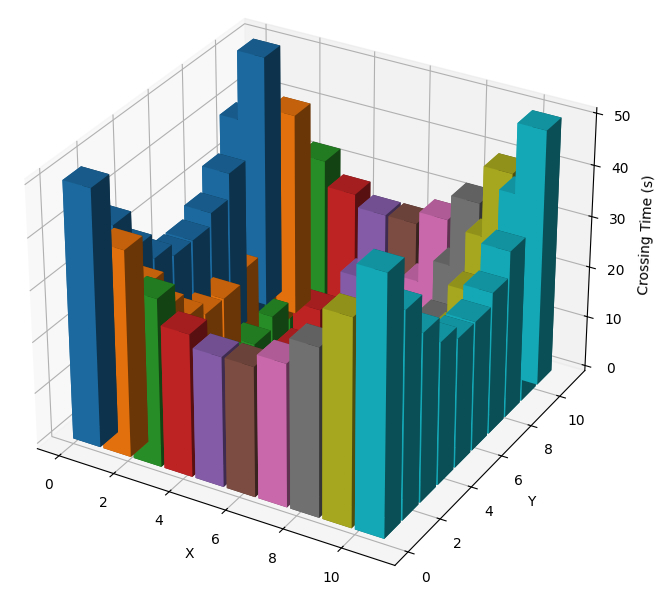
\includegraphics[width=5cm]{navfn-discrete.jpg} }}
    \qquad
    \subfloat[\centering Bicubic interpolation of navigation function]{{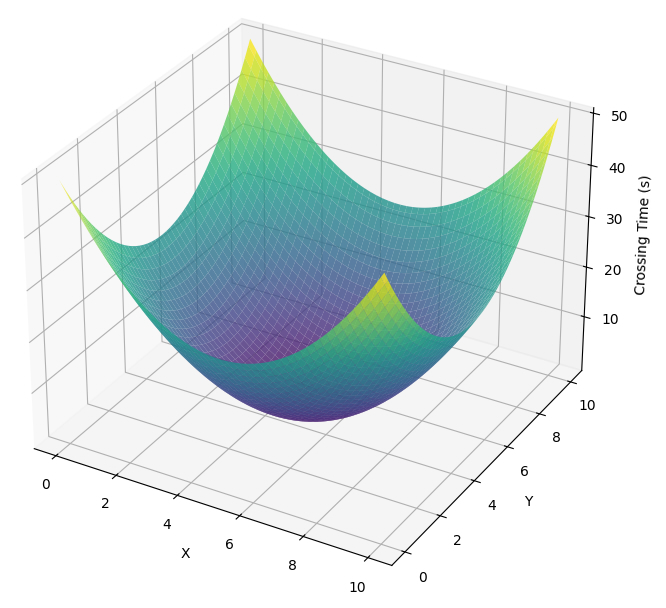
\includegraphics[width=5cm]{navfn-smooth.jpg} }}
    \caption{3D representation of how an example discrete navigation function is smoothed out for the gradient descent.}
    \label{fig:navfn}
\end{figure}

% A minimum travel cost is used so that the cost increases as the field propagates further.

\filbreak

\subsection{Local Path Planner} \label{local-planner}
After a path is generated by the global path planner, described in section \ref{global-planner}, the local path planner handles issuing linear and angular velocities ($v,\omega$) for the robot to follow the path \parencite{macenskiDesksROSMaintainers2023}. This planner serves to avoid new obstacles, make the path smoother, and keep movements steady. It uses the Dynamic Window Approach (DWA), which considers a range of physically possible linear and angular ``velocities that can be reached within the next time interval,'' as shown in Figure \ref{fig:dwa} \parencite{robotmaniaDynamicWindowApproach2020}. Many velocities would not be possible due to the limited torque exerted by the robot's motors. These parameters translate to circular arcs, which can be repeatedly adjusted every cycle to estimate the robot's intended path. All the paths generated by DWA are scored using the equation
\[
    \alpha heading(v,\omega) + \beta dist(v,\omega) + \gamma vel(v,\omega),
\]
where ``$heading(v,\omega)$ is a measure of distance to the goal, $dist(v,\omega)$ is the distance to the nearest obstacle on the trajectory, and $vel(v,\omega)$ encourages moving at full speed'' \parencite{macenskiDesksROSMaintainers2023}. These are called critic functions. $\alpha$, $\beta$, and $\gamma$ are constants used to change the weight of each critic function. In each cycle, the robot follows the path with the best score. ROS2 has many other integrated critic functions as well, including ``goal alignment,... path alignment, path distance, prefer forward motion, anti-twirling, anti-oscillation, and traversed cost by footprint or center value'' \parencite{macenskiDesksROSMaintainers2023}.

\begin{figure}[!htb]
    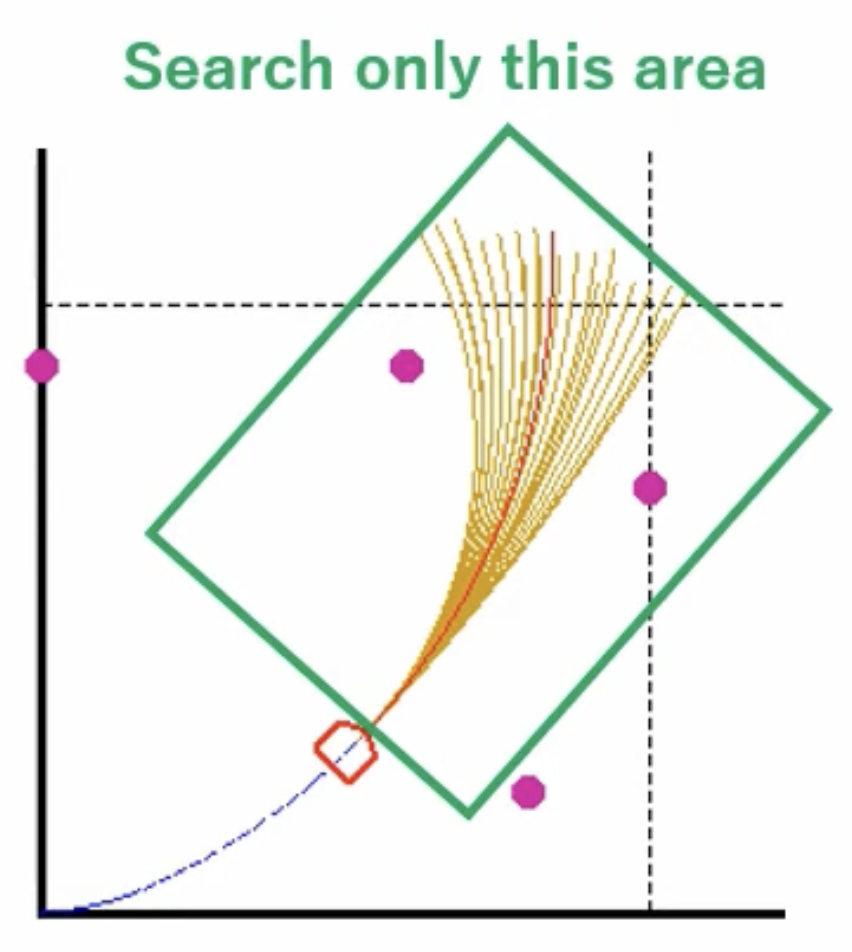
\includegraphics[width=6cm]{dwa.png}
    \centering
    \caption{Example of possible velocities considered by the Dynamic Window Approach (DWA) \parencite{robotmaniaDynamicWindowApproach2020}.}
    \label{fig:dwa}
\end{figure}


\section{Implementation and Testing} \label{implementation-and-testing}
As shown in Figure \ref{fig:map}, the mapping algorithm works well. This map was generated at Vanier College by manually driving the robot in an artificial environment. The environment was simply created by laying foldable tables and desk separators on the floor; thus, the obstacles used were big and could very easily be detected by the LiDAR sensor. While the mapping algorithm demonstrates promising results in a controlled environment, further testing in real-world settings is necessary.

Next, the Adaptive Monte Carlo Localization (AMCL) also works well. By providing the robot with an initial pose estimate within the pre-mapped environment, it can subsequently achieve precise and accurate localization after a brief period of motion. The repositioning of the robot in the map is very easily seen in RViz. Nevertheless, further testing with fully autonomous localization is needed.

Moreover, as of the time of writing this paper, there are still issues to be fixed with the global path planner. The robot is easily able to find and follow paths in large areas of free space; however, it cannot pass through narrower gaps. This is caused by the obstacles being too inflated. This can be simply fixed by changing the inflation parameter.

Lastly, the robot currently has issues with dead reckoning. As shown in Figure \ref{fig:dead-reckoning}, when moving towards a goal position with this navigation method, the robot stopped \qty{45}{cm} from the goal on the x-axis and \qty{35}{cm} from the goal on the y-axis. The percentage errors can be calculated as follows:
\begin{equation*}
    \begin{split}
        \% error_x & =\left|\frac{d_\text{experimental}-d_\text{actual}}{d_\text{experimental}}\right|\times100\%    \\
                   & =\left|\frac{(\qty{3}{m}-\qty{0.45}{m})-\qty{3}{m}}{\qty{3}{m}-\qty{0.45}{m}}\right|\times100\% \\
                   & =17.6\%
    \end{split}
\end{equation*}
\begin{equation*}
    \begin{split}
        \% error_y & =\left|\frac{d_\text{experimental}-d_\text{actual}}{d_\text{experimental}}\right|\times100\%          \\
                   & =\left|\frac{(\qty{0.6}{m}-\qty{0.35}{m})-\qty{0.6}{m}}{\qty{0.6}{m}-\qty{0.35}{m}}\right|\times100\% \\
                   & =140\%
    \end{split}
\end{equation*}
These significant errors are causes by two factors. First, there is wheel slippage die to the very smooth floor. Thus, a rougher floor may improve the results. Second, the dead reckoning algorithm produces very low wheel velocities at the beginning and end of the trajectory. Since these velocities are rounded to 0, the robot does not move and error is introduced. A solution addressing this problem has yet to be found.

\begin{figure}[!htb]
    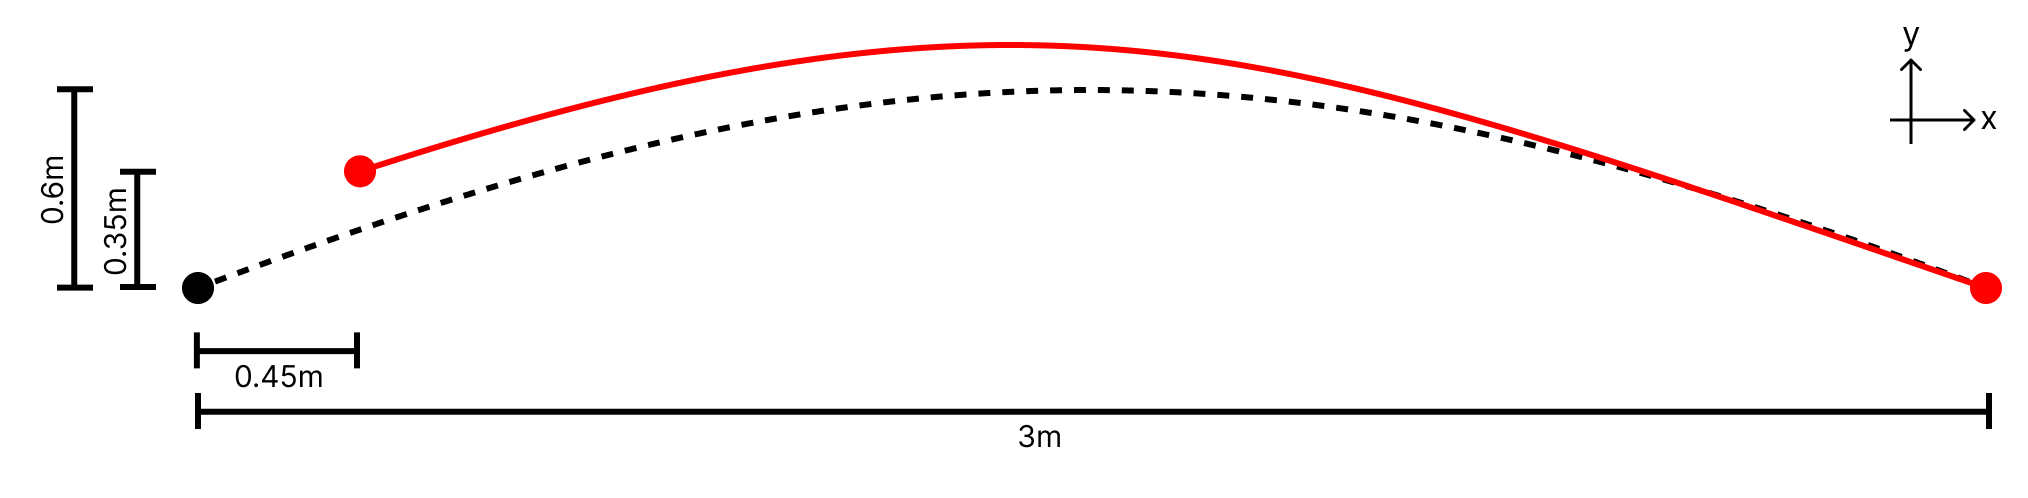
\includegraphics[width=12cm]{dead-reckoning.jpg}
    \centering
    \caption{Representation of the dead-reckoning test. The black dotted path is the intended path, while the red continuous path is the actual path of the robot.}
    \label{fig:dead-reckoning}
\end{figure}

\section{Conclusion} \label{conclusion}
In conclusion, this project achieved its core objectives by developing a robot that can map its environment, localize itself within the map, and navigate large open spaces. While some refinements are necessary, particularly with the global path planner and dead reckoning, these issues do not significantly impact the robot's overall performance. More importantly, this project introduces the fundamentals of SLAM and autonomous navigation, which can be used for the development more complex robots in the future.

\newpage
\section*{Acknowledgments} \label{acknowledgments}
I would like to express my sincere gratitude to Professors Ivan T. Ivanov, Christian Stahn, and Kevin James Lenton for their invaluable guidance and support throughout this project. Their expertise in mathematics, physics, and robotics proved instrumental in not only bringing the robot to life but also in shaping the research presented in this paper.

\newpage
\printbibliography

\end{document}